%------------------------------------------------------------------------------

\typeout{UTK Thesis Style: Modified by David L. Page}

% To use different formats, simply uncomment the lines relative to the 
% following option's labels. Note that only this main file contains 
% section that need to be uncommented.
%
% Option1: Doubled-sided, open-right format.
% Option2: Doubled-sided format.
% Option3: Single-sided format.
%------------------------------------------------------------------------------

\documentclass[letterpaper,twoside,11pt,openright,pdf]{book} % Option1
%\documentclass[letterpaper,twoside,11pt]{report} %Option2
%\documentclass[letterpaper,11pt]{report} %Option3

% Load some packages (may need to download)
\usepackage[pdftex]{graphicx}             % Graphics formats
\usepackage{amsmath,amssymb}             % AMS Math
\usepackage{fancyhdr}                    % Fancy Headers and Footers
\usepackage{setspace}                    % Line spacing
\usepackage{subfigure}                   % Nice subfigures
\usepackage{cite}                        % Nice citations
\usepackage{url}                         % Nicely format url breaks
\usepackage[vcentering,dvips]{geometry}  % Help with margins

% Set margins appropriately
\geometry{twoside} % Option1 & Option2
\geometry{
    letterpaper,
    left=   1.5in,
    right=  1.0in,
    top=    1.0in,
    bottom= 1.0in
}

% Give directory where figures are located
\graphicspath{{figs/}}

% Over-ride Latex hyphenation
\hyphenation{pa-ra-me-ter}%


% Widow/orphan protection
\clubpenalty=10000    % Minimize orphans orphans(eliminate 10000)
\widowpenalty=10000   % Minimize widows
\brokenpenalty=10000  % Do not allow hyphen across pages


% Use cool footnotes
\renewcommand{\thefootnote}{\fnsymbol{footnote}}

% Allow empty pages before chapters (i.e. no page numbers)
\makeatletter
\let\origdoublepage\cleardoublepage
\newcommand{\clearemptydoublepage}{%
  \clearpage
  {\pagestyle{empty}\origdoublepage}%
}
\let\cleardoublepage\clearemptydoublepage
\makeatother

% Set some figure placement parameters
\renewcommand{\topfraction}{.85}
\renewcommand{\bottomfraction}{.7}
\renewcommand{\textfraction}{.5}
\renewcommand{\floatpagefraction}{.35}
\renewcommand{\dbltopfraction}{.66}
\renewcommand{\dblfloatpagefraction}{.66}
\setcounter{topnumber}{9} %
\setcounter{bottomnumber}{9} %
\setcounter{totalnumber}{20} %
\setcounter{dbltopnumber}{9}

%  Prints your review date and 'Draft Version' (From Josullvn, CS, CMU)
\newcommand{\reviewtimetoday}[2]{
    \special{!userdict begin
        /bop-hook{
             gsave
                 20 710 translate
                 45 rotate
                 0.8 setgray
                 /Times-Roman findfont
                 12 scalefont
                 setfont
                 0 0 moveto
                 (#1) show
                 0 -12 moveto
                 (#2) show
             grestore
        } def end
    }
}

% You can turn on or off this option.
%\reviewtimetoday{\today}{Draft Version}

\raggedbottom
\doublespacing%
\pagestyle{plain}

%------------------------------------------------------------------------------
\def\eqstart{\begin{equation}}
\def\eqend{\end{equation}}

\title{Solving the Two-Dimensional Euler Equation using a Point-Iterative Linear Solve and Green's Theorem Gradients}
\date{April 19, 2007}
\author{Vincent Charles Betro}
\begin{document}

\maketitle

\pagenumbering{arabic} %
\setcounter{page}{1}

\begin{center}
\textbf{Abstract}
\end{center}

One subset of the Navier-Stokes equations is the Euler Equations.  Despite the fact that these are non-linear in nature, they can be solved using an LU-factorization by linearizing the fluxes.  The use of the chain rule in creating analytic flux jacobians, Cuthill-McKee reordering in clustering non-zero values about the diagonal, and CFL ramping to allow for more correct gradient calculation are all key elements of the approach taken.  The end product was a second order implicit solver run on a NACA0012 airfoil as a test case.

\begin{center}
\textbf{Nomenclature}
\end{center}

\begin{center}
\begin{table}[htbp]
\centering
\begin{tabular}{ll}
\(\Omega\) & A control volume \\
\(\Gamma\) & The boundary of a control volume \\
\(\vec{F}\) & The flux over a control volume \\
\(\vec{n}\) & The unit normal pointing out of the control volume at a given face \\
\(Q\) & A vector composed of density, x-y momentum, and total energy at a given node \\
\(\rho\) & Density at a given node \\
\(u\) & X velocity at a given node \\
\(v\) & Y velocity at a given node \\
\(e_t\) & Total energy at a given node \\
\(e_i\) & Internal energy at a given node \\
\(\gamma\) & Specific gravity (here, assumed to be 1.4) \\
\(c\) & Speed of sound in air \\
\(\bar{u}\) & Magnitude of the velocity vector \\
\(p\) & Pressure \\
\(R_i\) & Residual \\
\(\alpha\) & Angle of attack \\
\end{tabular}
\end{table}
\end{center}

\section{Introduction}

One primary aim of the study of Computational Fluid Dynamics is to solve the Navier-Stokes equations using numerical techniques (Anderson07).  To that end, one of the model equations that can be used as a building block is the two-dimensional inviscid Euler Equation: 
\eqstart
\frac{\delta}{\delta t}\int_\Omega Q d\Omega + \int_\Gamma \vec{F}\cdot \vec{n} d\Gamma = 0
\label{eulerint}
\eqend
where \(\Omega\) is a control volume, \(\Gamma\) is the boundary of the control volume, and \(\vec{n}\) is the unit normal pointing out of the control volume at a given face.  In the two-dimensional version of Equation \ref{eulerint}, \(Q\) is a vector of the mass, x-y momentum, and energy per unit volume as follows:
\[Q = \left[ \begin{array}{c} \rho \\ \rho u \\ \rho v \\ e_t \end{array} \right] \]
and \(\vec{F}\) is the flux over the faces, both viscous and inviscid.  Here, since we are using the Euler Equation, only the inviscid aspects will be discussed.

To discretize Equation \ref{eulerint}, Backward Euler is used for the time derivative. It should be noted here that VanLeer flux vector splitting is used.  As a consequence, the flux vector is split as such for the left and right states for subsonic flow (non-dimensionalized):
\eqstart
\vec{F}^{\pm} \cdot \vec{n} = \left[ \begin{array}{c} \pm \frac{1}{4} \rho c \left(\frac{\bar{u}}{c} \pm 1 \right)^2 \\ F_1^{\pm} \left(\frac{\vec{n}_x}{\gamma}(-\bar{u} \pm 2c) + u \right) \\ F_1^{\pm} \left(\frac{\vec{n}_y}{\gamma}(-\bar{u} \pm 2c) + v \right) \\ F_1^{\pm} \left( \frac{(-(\gamma - 1)\bar{u}^2 \pm 2(\gamma - 1)\bar{u}c + 2c^2)}{\gamma^2 - 1} + \frac{(u^2+v^2)}{2} \right) \end{array} \right]
\label{fplusminus}
\eqend
where \(c\) is the speed of sound and \(\bar{u} = \vec{n}_x u + \vec{n}_y v\).  If the magnitude of the velocity of the node to the left of the face is supersonic and flowing out of the control volume, then \(\vec{F}^+\) becomes (non-dimensionalized):
\eqstart
\vec{F}^{+} \cdot \vec{n} = \left[ \begin{array}{c} \rho \bar{u} \\ \rho u \bar{u} + \vec{n}_x p \\ \rho v \bar{u} + \vec{n}_y p \\ (e+p)\bar{u} \end{array} \right]
\label{fplusminussonic}
\eqend
This is identical to the change in \(\vec{F}^-\) when the magnitude of the velocity of the node to the right of the face is supersonic and flowing into the right node's control volume.  In both cases, the opposite signed \(\vec{F}\) is \(\vec{0}\) (VanLeer82).  

Also, the fluxes on the far-field boundaries were taken to be free-stream (zero) and those at the inner, inviscid boundaries were taken to be of the form:
\eqstart
F = \left[ \begin{array}{c} 0 \\ \vec{n}_x p \\ \vec{n}_y p \\ 0 \end{array} \right].
\label{fbd}
\eqend

The integral of the fluxes through the faces of each control volume is computed by cycling through the faces and summing the appropriately signed component (positive normal always points \textit{out} of the control volume) to the residual of each node.  The only caveat is that in order to close off the boundary segments, a three-quarters share is taken from the closer node and a one-quarter share from the further node, using the flux from Equation \ref{fbd}.  This sum for each node will be denoted from here on as \(R_i\).  

Since the code can be run both first and second order implicit, it should be noted that when running second order, the extrapolated values of \(Q\) (see Equation \ref{grad}) are used to evaluate the fluxes, where \(\vec{r}\) is the distance from the node to the midpoint of the face.  Since these extrapolated values are used to reconstruct \(Q\), Linear Least Squares would have been the best method for computing gradients due to its ability to give a more accurate reconstruction (Anderson07).  Here, Green's Theorem was used to generate the gradients, yet the extrapolated values still provided good results.

\eqstart
\vec{Q}_{face} = \vec{Q}_{node} + \nabla\vec{Q}_{node}\cdot\vec{r}
\label{grad}
\eqend

Thus, our discretized, implicit equation takes the following shape:
\eqstart
A\left(\frac{Q_i^{n+1} - Q_i^n}{\Delta t}\right) + R_i^{n+1} = 0
\label{eulerdiscr}
\eqend
However, the values of the fluxes at the \(n+1^{th}\) time step are not known, so Taylor Series must be used to derive the following expression for \(R_i^{n+1}\):
\eqstart
R_i^{n+1} = R_i^n + \sum\frac{dR_i}{dQ_j}\Delta Q_i^n
\label{Rtaylor}
\eqend
where \(j\) is a neighboring node (that shares an edge).  Substituting Equation \ref{Rtaylor} into Equation \ref{eulerdiscr} and noting that \(\Delta Q = Q^{n+1} - Q^n\), the result is:
\eqstart
\left(\frac{A}{\Delta t} + \sum\frac{dR_i}{dQ_j}\right)\Delta Q_i^n = -R_i^{n}
\label{euler final}
\eqend

The quantity \(\frac{dR_i}{dQ_j}\) is obtained by taking the derivative of each primitive variable in \(Q\) with respect to each element in \(Q\).  For example, \(\frac{d\rho}{dQ}\) would be the following vector:

\[\left[ \begin{array}{c} 1.0 \\ 0.0 \\ 0.0 \\ 0.0 \end{array} \right] \].

Now, the derivative of each element in the flux (Vectors \ref{fplusminus} and \ref{fplusminussonic}) is taken with respect to each of the primitive variables, and the chain rule is applied as such for the case of \(\rho\) (Anderson07):

\[\frac{dR}{dQ} = \frac{dR}{d\rho}\frac{d\rho}{dQ}\].

\section{Implementation}

In order to implement this scheme numerically, a valid mesh was needed and initial free-stream values from which to initialize the flow field.  An angle of attack in radians, \(\alpha\), and velocity, \(Mach\) number, were input from which the following non-dimensionalized values were obtained to place in the previous equations:
\[\rho = 1\]
\[c = 1\]
\[p = \frac{\rho c^2}{\gamma}\]
\[u = Mach\,cos(\alpha)\]
\[v = Mach\,sin(\alpha)\]
\[e_i = \frac{p}{(\gamma-1)\rho}\]
\[e_t = \rho(e_i+\frac{1}{2}(u^2+v^2))\]

In order to non-dimensionalize, the following equivalences were used , where the hat denotes the non-dimensionalized value and the infinity denotes the reference value for the given problem:
\[\hat{\rho} = \frac{\rho}{\rho_{\infty}}\]
\[\hat{c} = \frac{c}{c_{\infty}}\]
\[\hat{p} = \frac{p}{\rho_{\infty}c^2_{\infty}}\]
\[\hat{u} = \frac{u}{u_{\infty}}\]
\[\hat{v} = \frac{v}{v_{\infty}}\]
\[\hat{e_i} = \frac{e_i}{c^2_{\infty}}\]
\[\hat{e_t} = \frac{e_t}{c^2_{\infty}}\]

Equation \ref{euler final} will yield a large, sparse matrix of \(4\times4\) submatrices that will look like Matrix \ref{mat} using C++ indexing:
\eqstart
\left[
\begin{array}{ccccc}
D_0 & \frac{dR_0}{dQ_1} & \dots & \frac{R_0}{dQ_{nn-2}} & \frac{R_0}{dQ_{nn-1}} \\
\frac{dR_1}{dQ_0} & D_1 & \dots & \frac{R_1}{dQ_{nn-2}} & \frac{R_1}{dQ_{nn-1}} \\
\vdots & \vdots & \vdots & \vdots & \vdots \\
\frac{dR_{nn-2}}{dQ_0} & \frac{dR_{nn-2}}{dQ_1} & \dots & D_{nn-2} & \frac{R_{nn-2}}{dQ_{nn-1}} \\
\frac{R_{nn-2}}{dQ_0} & \frac{R_{nn-2}}{dQ_1} & \dots & \frac{R_{nn-1}}{dQ_{nn-2}} & D_{nn-1} \\
\end{array}
\right] 
\left[
\begin{array}{c}
x_0 \\ x_1 \\ \dots \\ x_{nn-2} \\ x_{nn-1}
\end{array}
\right]
=
\left[
\begin{array}{c}
R_0 \\ R_1 \\ \dots \\ R_{nn-2} \\ R_{nn-1}
\end{array}
\right]
\label{mat}
\eqend
where \(D_i\) is a \(4\times4\) with the additional \(\frac{A}{\Delta t}\) on the diagonal and \(\frac{dR}{dQ}\) is a \(4\times4\) analytic flux jacobian matrix.

However, in order to save memory, a compressed row storage routine was used (Anderson07).  In order to generate this compressed row storage, the \verb+ja+ array was created, which is the node to node hash table compressed into one array.  Thus, the number of non-zero entries in Matrix \ref{mat} are now known and a compressed version of Matrix \ref{mat} can be dimensioned which will hereafter be called \verb+mat+. The three-dimensional matrix \verb+mat+ will have as its first dimension the number of entries in \verb+ja+ and the next two dimensions of 4 and 4, since each node in the hash table will have a corresponding \(4\times4\) submatrix.  Each partition of \verb+mat+ can be accessed by creating the \verb+ia+ array, which holds the beginning index of each incomplete ``row'' in Matrix \ref{mat}.  Finally, the \verb+iau+ array is generated, which holds the locations in the \verb+mat+ matrix of the diagonal entries in the Matrix \ref{mat}.

When creating the control volumes, the median-dual style control volume was used (Anderson07).  This creates a control volume (red lines in Figure \ref{fig:md}) around a point (blue node in Figure \ref{fig:md}) such that the edges are composed of segments emanating from each triangle's edge midpoint and connecting to its centroid.

\begin{center}
\begin{figure}[h]
\centering
\scalebox{0.5}[0.5]{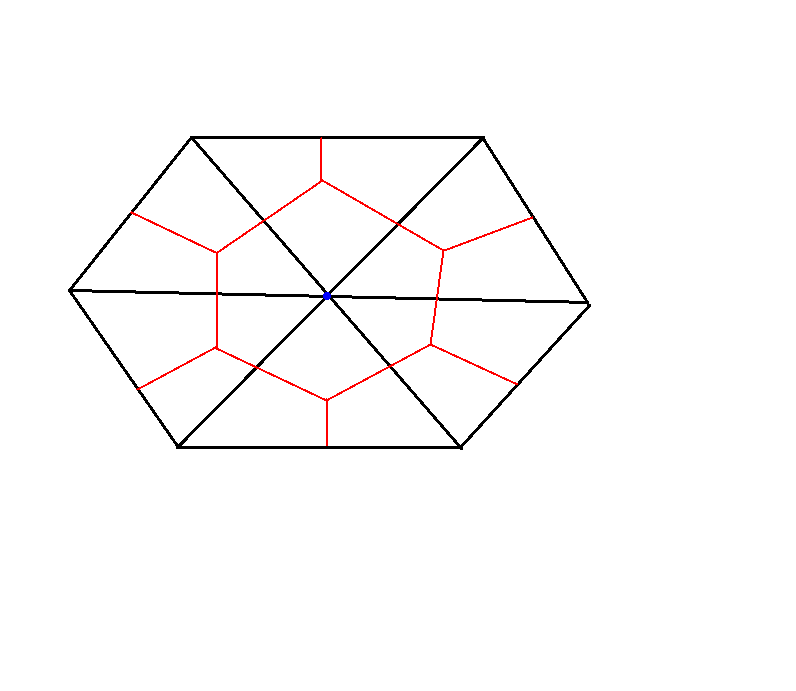
\includegraphics{mediandual.png}}
\caption{An example median-dual control volume (in red) for the blue node.}
\label{fig:md}
\end{figure}
\end{center}

In building the left hand side matrix, a value for \(\Delta t\) was required, except on the boundaries, where the entire diagonal was initialized to ones.  Since \(\Delta t\) varies by node, it was obtained from the following formula:
\[ \Delta t = \frac{CFL*len}{|\bar{u}| + c} \]
where \(len\) is the perimeter of the control volume and \(c = \sqrt{\frac{\gamma p}{\rho}}\).

In order to solve Equation \ref{euler final}, a Point-Iterative solver was used with symmetric Gauss-Seidel updating and LU-factorization with forward and back substitution.  First, the off-diagonal submatrices of each row were transfered to the corresponding right-hand side (where \(R_i\) resides) by multiplying them by the values of the current solution (at time \(n\)) and subtracting the result from \(R_i\), which will be called \(R_i^*\).  Then, the system composed of a diagonally dominant \(4\times4\), due to the addition of the \(\frac{A}{\Delta t}\) term, and \(R_i^*\) is solved using LU-factorization to obtain the value of the solution at a given node at time \(n+1\).  The RMS error was computed at the end of each time step using the following formula:
\eqstart
RMS = \frac{\sum_{i=0}^{nn}(R_i^* - D_i*x_i)^2}{nn}
\label{RMS}
\eqend

Additionally, in order to cluster the dependent nodes that each node has as nearest neighbors along the diagonal of Matrix \ref{mat}, which yields a faster solve since more updated values are available as the matrix is cycled through, Cuthill-McKee Reordering was used (Cuthill80).  This, along with using symmetric Gauss-Seidel updating in the Point-Iterative solve, allows the most updated values of \(Q\) to be used for each step of the linear solve, and speeds convergence.

\section{Results} 
The following results are based on a 4156 node, Delauney mesh around a NACA0012 airfoil.  Second order spatial accuracy was used and ran for 1000 external iterations (such that the values of \(Q\) are updated from the \(\Delta Q\) obtained from solving Equation \ref{euler final} in between each iteration) or until reaching an RMS error of \(1.0e-15\).

One of the tests that was run was to vary the number of iterations of the Point-Iterative solve (which solves for \(\Delta Q\) in Equation \ref{euler final}) that could be done before the update of \(Q\).  Using lower numbers of point-iterative iterations than the choices given in the application before updating \(Q\) could have caused the update directions to be wrong, and thus the system would not converge.  Since symmetric Gauss-Seidel was used, these errors would propagate very quickly.

The less point-iterative iterations that are used, the quicker the system will converge in time but with more non-linear iterations (see Figure \ref{fig:RMSI}).  As more iterations are added in the Point-Iterative loop, the convergence takes less non-linear iterations, but significantly more time, since the changes in the \(\Delta Q\) obtained from the Point-Iterative solve after more than 5 internal iterations become drastically less significant.

\begin{center}
\begin{figure}[h]
\centering
\scalebox{0.5}[0.5]{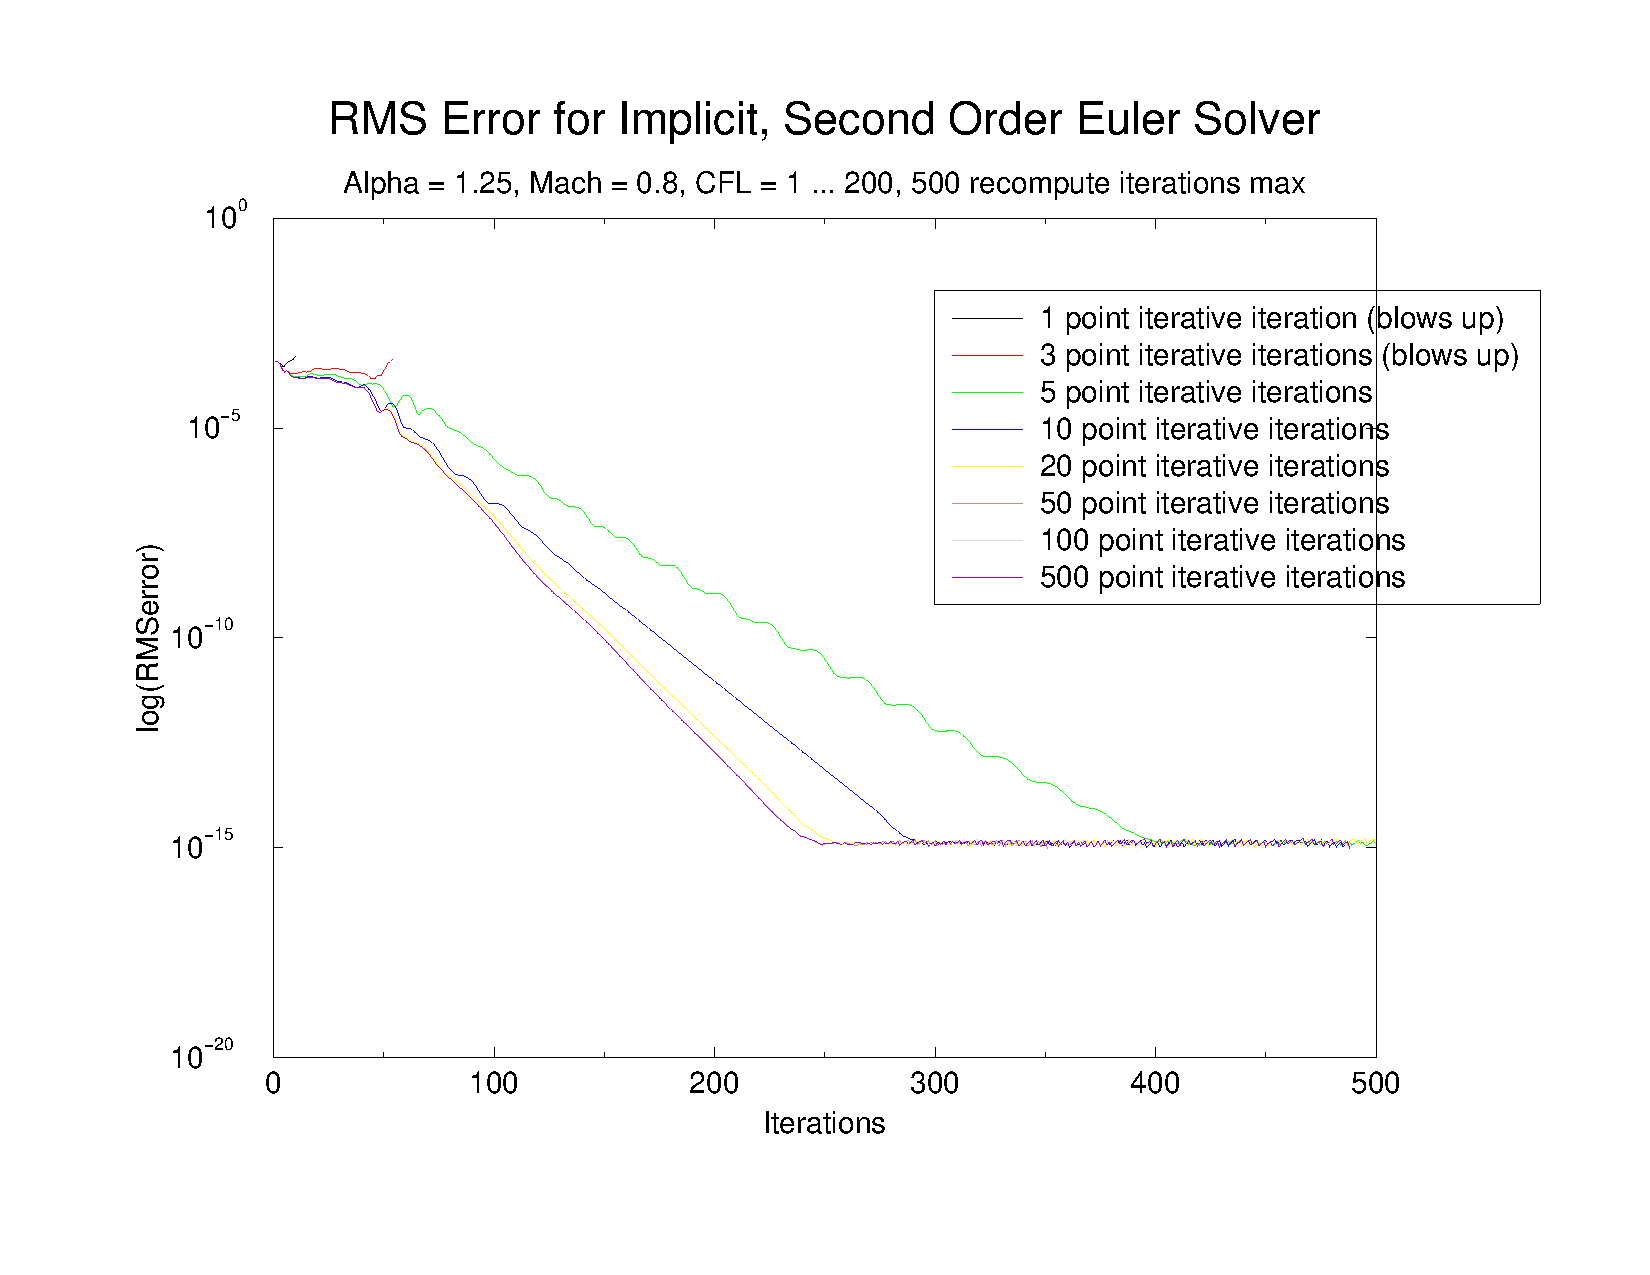
\includegraphics{RMSiterative.pdf}}
\caption{RMS error versus iterations for second order solve at varying numbers of Point-Iterative iterations}
\label{fig:RMSI}
\end{figure}
\end{center}

The maximum CFL is given as an input value and ramped up from 1 over 100 iterations using Formula \ref{ramp}.  

\eqstart
CFL = CFL_{init} + \frac{iteration - 1}{99}(CFL_{max} - CFL_{init})
\label{ramp}
\eqend

As one can see in Figure \ref{fig:RMST}, the low CFL numbers took the longest to converge, and a CFL of 500 had the most rapid convergence.  The cases with CFL numbers of 1500 and 2500 failed to converge, and thus were not given as options in this application.  This is due to the fact that the gradients are changing so rapidly in the second-order solve that the initial time stepping must be slowed down for a while to catch all the changes accurately, without yielding negative densities and pressures or causing zeros to appear on the diagonals of the flux jacobians. Once this change in gradients slows down, the CFL can be quickly raised and remain there to get a more rapidly converged answer.

\begin{center}
\begin{figure}[h]
\centering
\scalebox{0.5}[0.5]{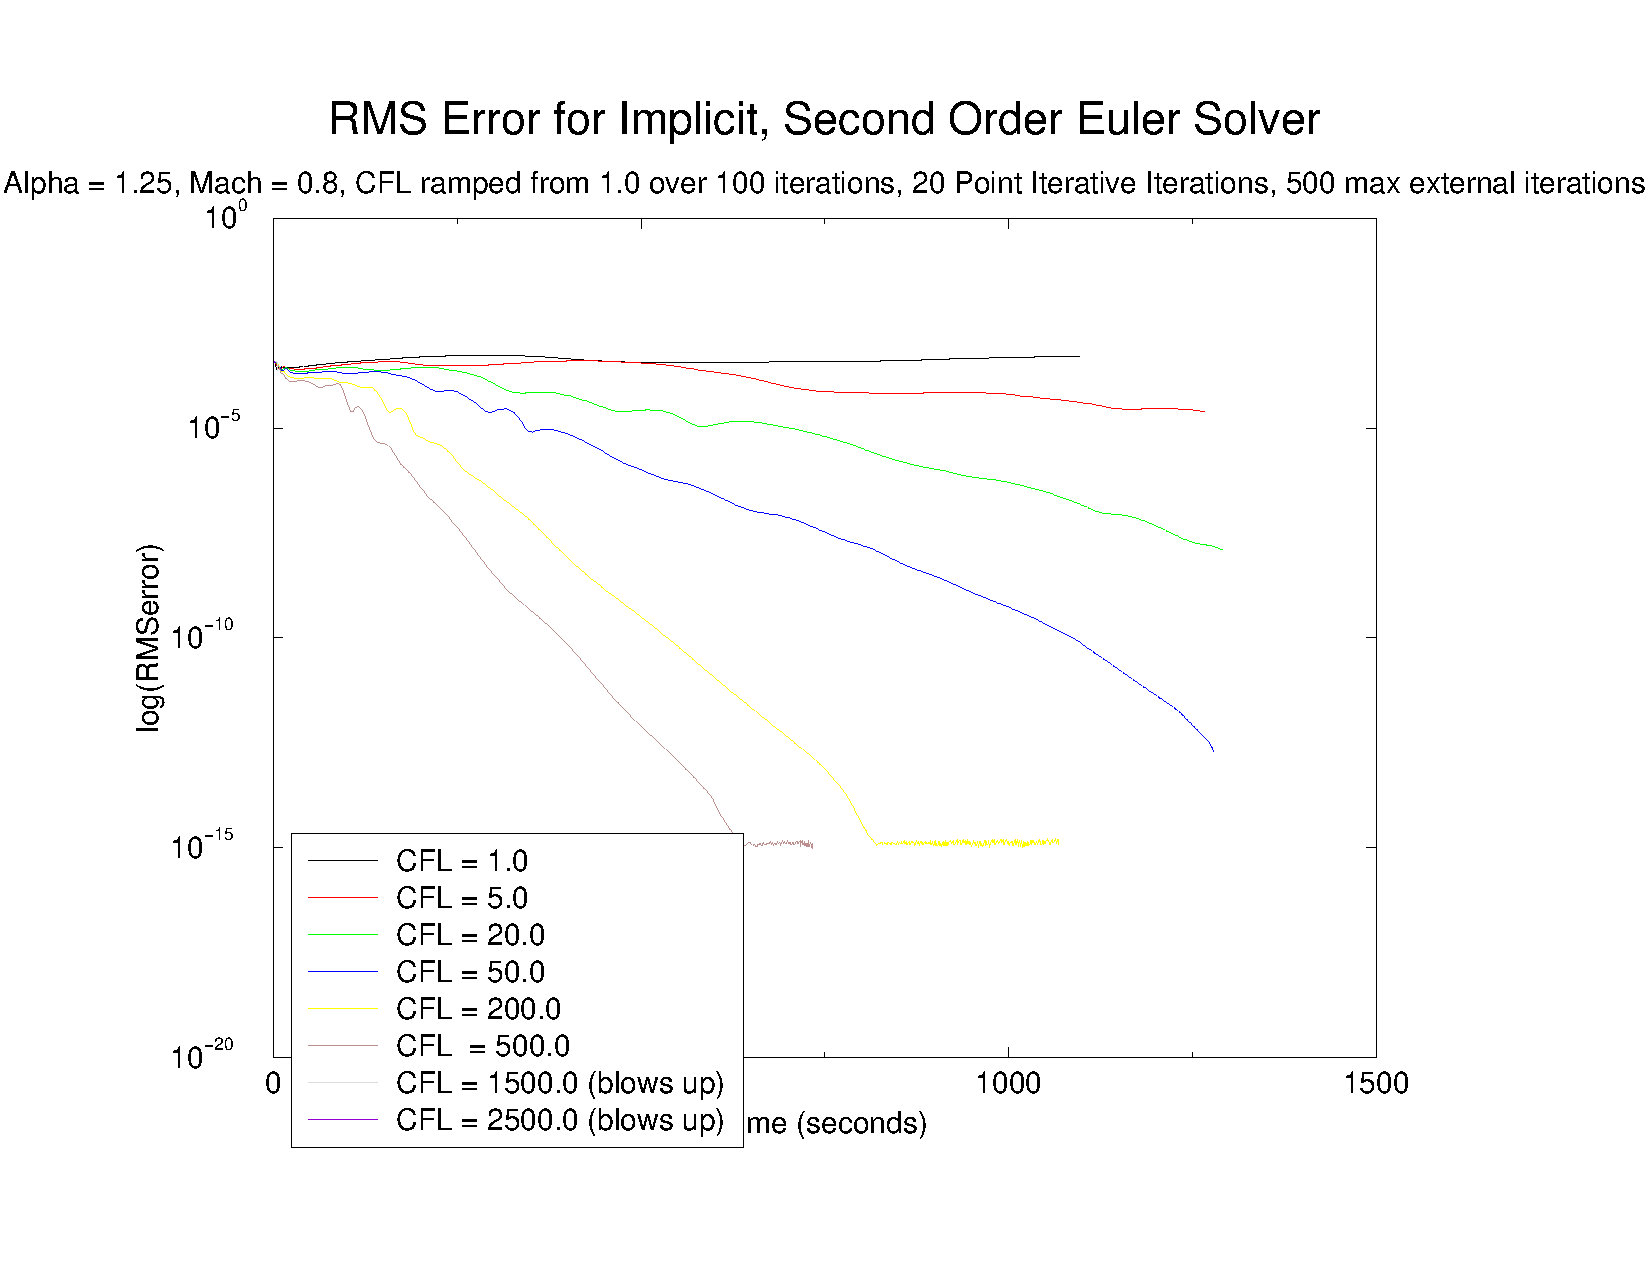
\includegraphics{RMScT.pdf}}
\caption{RMS error versus time for second order solve at varying maximum CFL numbers}
\label{fig:RMST}
\end{figure}
\end{center}

In cases where an initial second order solve was not possible, a first order solve was run for 100 iterations, allowing the gradients o change more slowly and by lower magnitudes.  Thus, the negative pressures and densities were avoided that would have caused zeros on the diagonal and thus failure to converge due to the poorly constructed flux jacobians.  Once the gradients stopped changing as rapidly, the process continued on with a second order run and dissipation occurred in the results as expected. 

Additionally, the resemblance to the physical realities of shocks on an airfoil garnered from the solver was quite good despite the absence of flux limiters (which would alleviate the extra spikes seen in Figure \ref{fig:CP}).  The shocks are displayed for both the top and bottom of the airfoil in the appropriate spots in terms of both coefficient of pressure and flow density, in Figures \ref{fig:CP} and \ref{fig:RHO}, respectively.

\begin{center}
\begin{figure}[h]
\centering
\scalebox{0.5}[0.5]{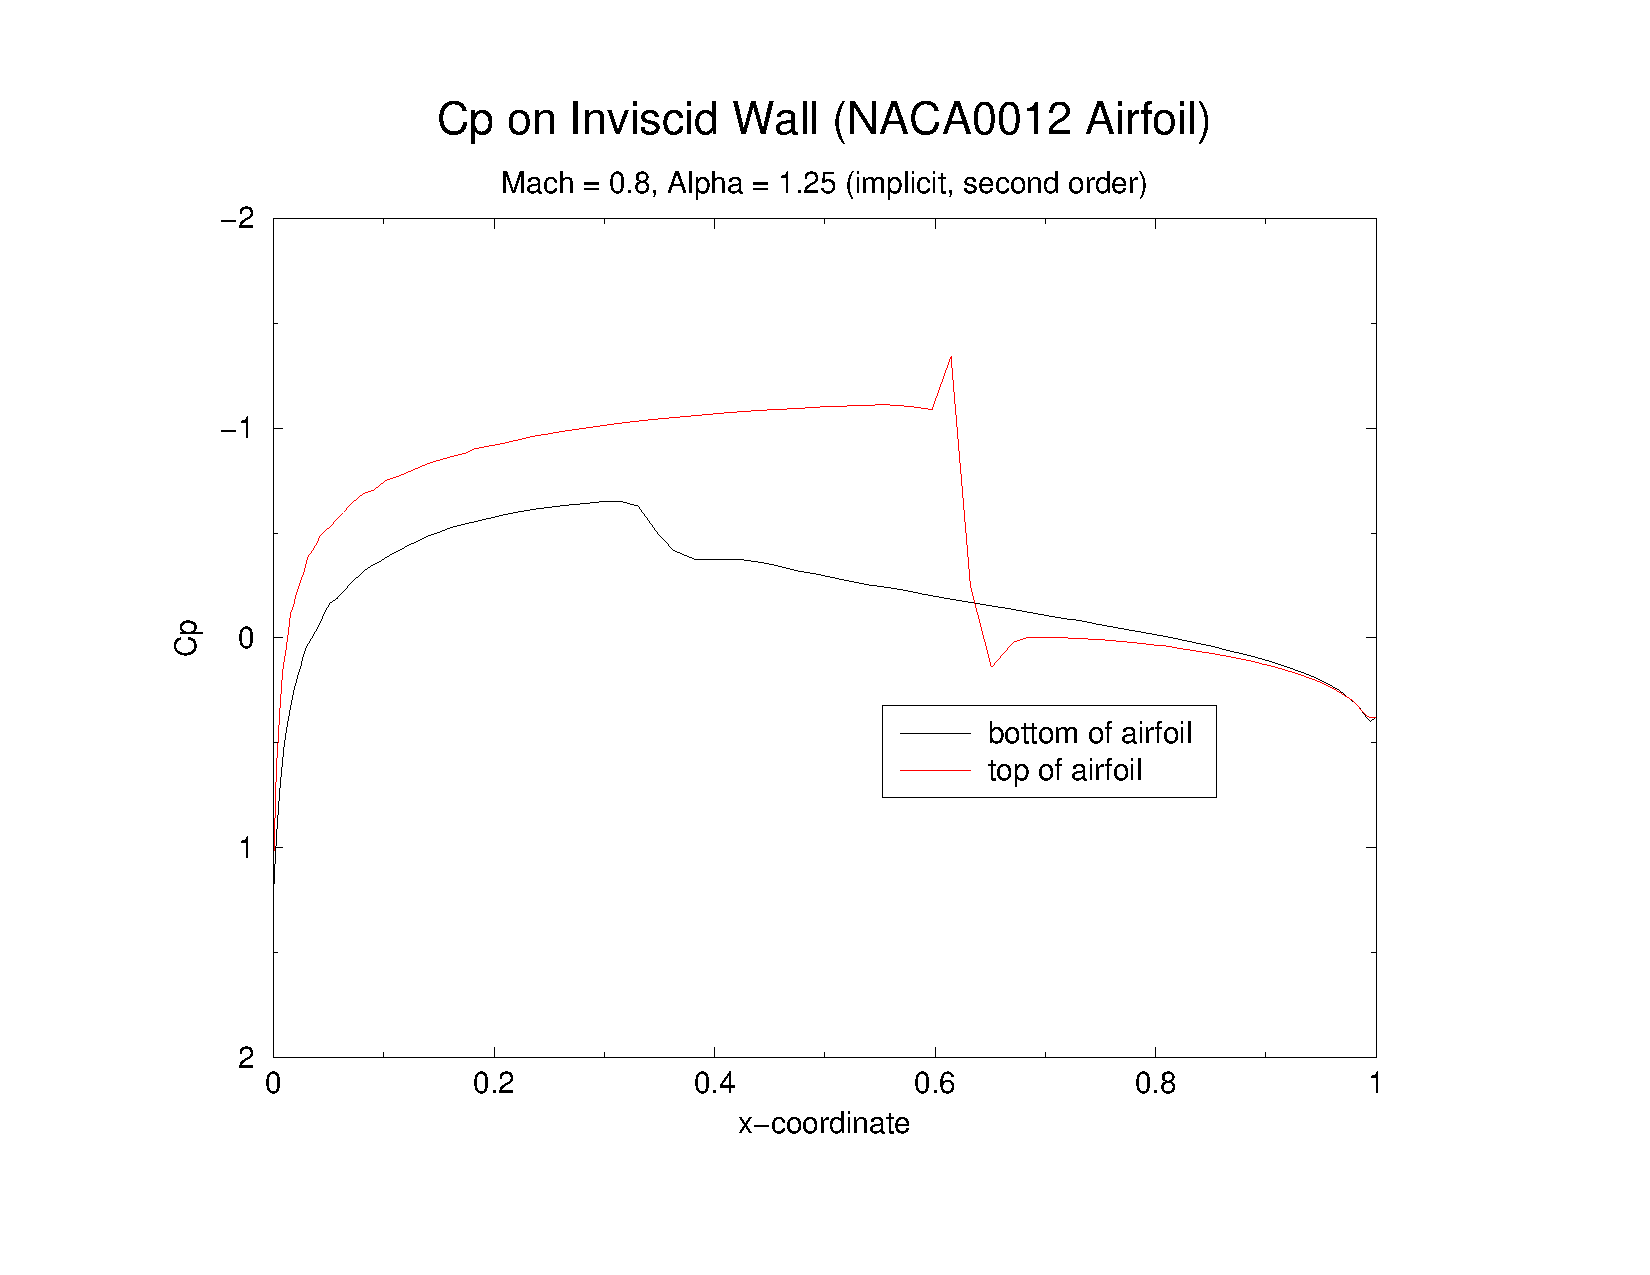
\includegraphics{Cp2.pdf}}
\caption{Coefficient of Pressure for NACA0012 airfoil, obtained from second order solve at Mach=0.8, Alpha = 1.25}
\label{fig:CP}
\end{figure}
\end{center}

\begin{center}
\begin{figure}[h]
\centering
\scalebox{0.5}[0.5]{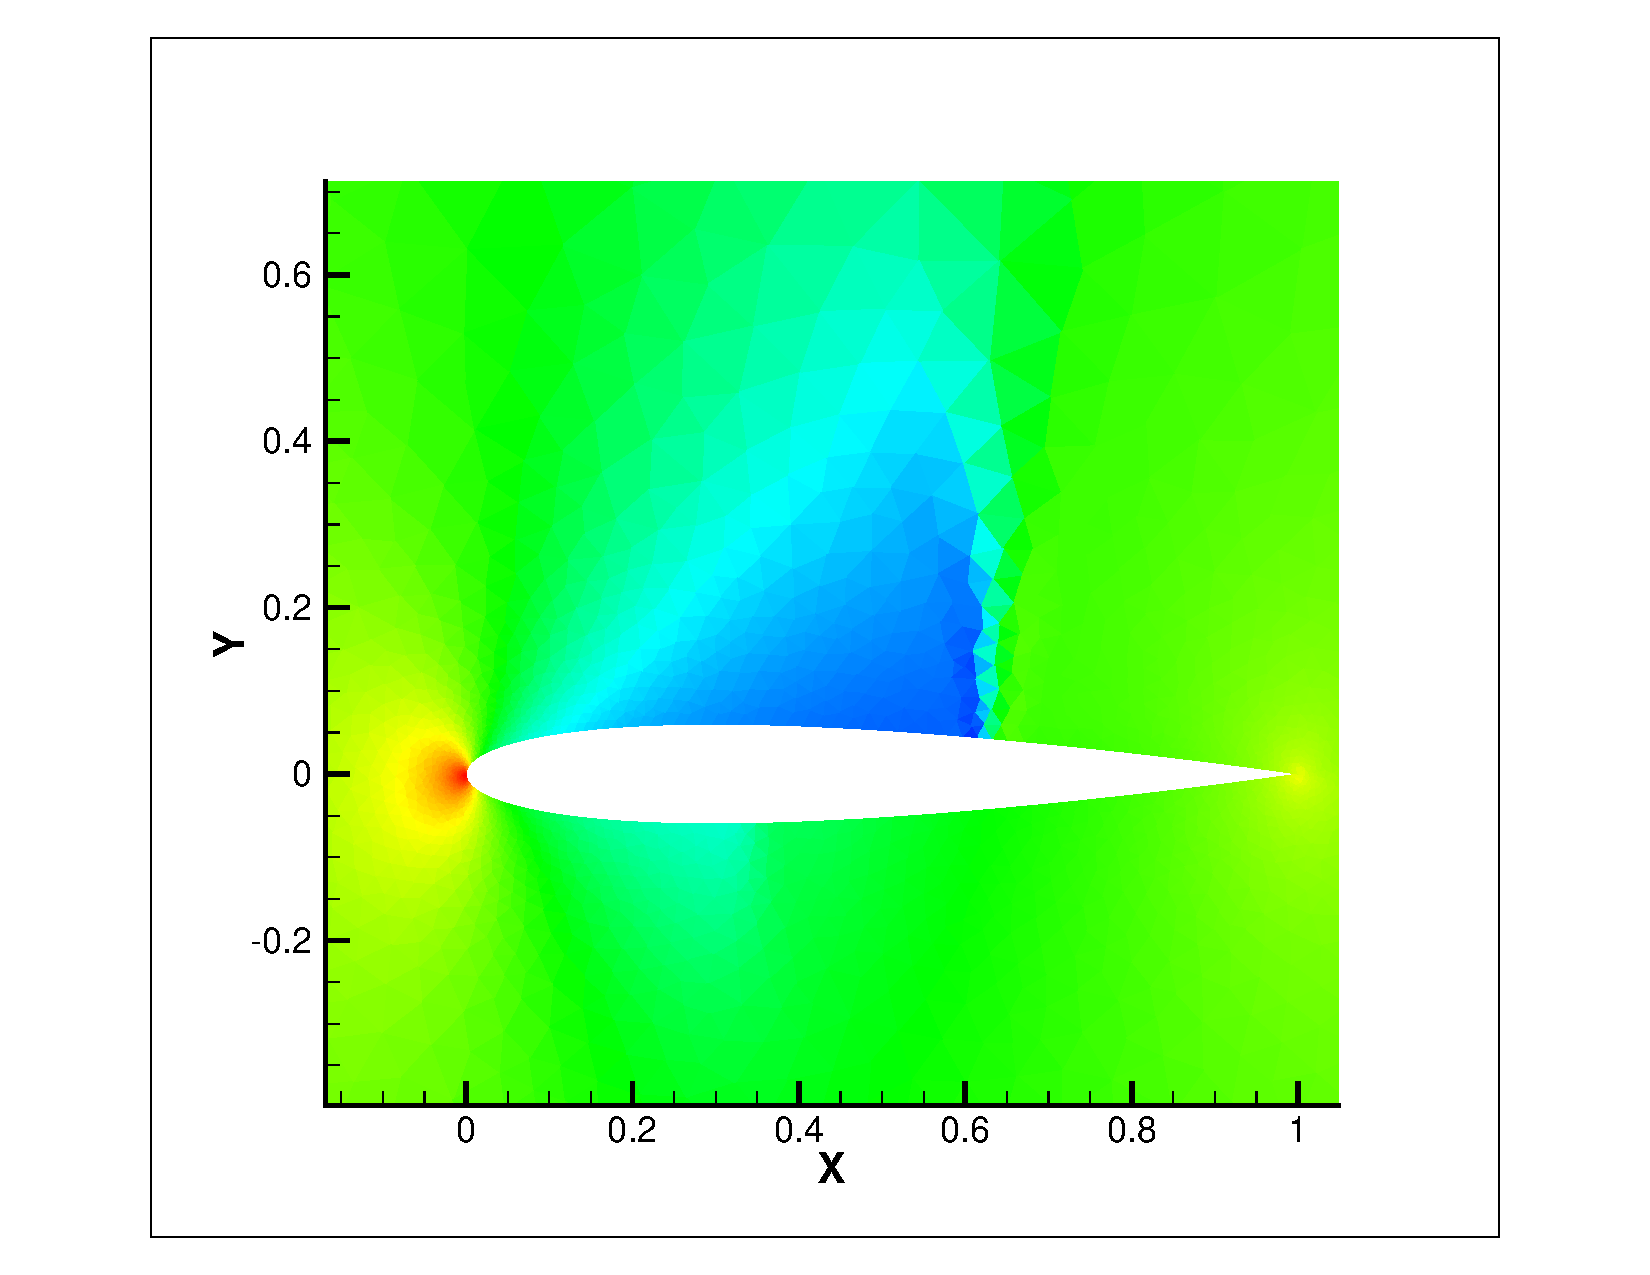
\includegraphics{rho.pdf}}
\caption{Density contours for NACA0012 airfoil, obtained from second order solve at Mach=0.8, Alpha = 1.25}
\label{fig:RHO}
\end{figure}
\end{center}

\begin{center}
\textbf{Conclusions}
\end{center}

Using a reasonable amount of computing power, solutions that emulate reality were found in regards to shocks and pressure coefficient data on a NACA0012 airfoil.  By adding such elements as flux limiters and better approximations of viscous flow over the boundaries, even better results will be achieved.  However, such novel ideas as compressed row storage and chain rule analytic flux jacobians proved invaluable in the solution of the Euler Equations.
 
\bibliographystyle{apalike}
\bibliography{page-bib-abbr,page-bib-refs}


\end{document}
%------------------------------------------------------------------------------
